%%%%%%%%%%%%%%%%%%%%%%%%%%%%%%%%%%%%%%%%%
% Structured General Purpose Assignment
% LaTeX Template
%
% This template has been downloaded from:
% http://www.latextemplates.com
%
% Original author:
% Ted Pavlic (http://www.tedpavlic.com)
%
% Note:
% The \lipsum[#] commands throughout this template generate dummy text
% to fill the template out. These commands should all be removed when 
% writing assignment content.
%
%%%%%%%%%%%%%%%%%%%%%%%%%%%%%%%%%%%%%%%%%

%%%%%%%%%%%%%%%%%%%%%%%%%%%%%%%%%%%%%%%%%
%TODO
% 
% USE CASE (of vervanging hiervan)
% SUBSYSTEEM DECOMPOSITIE
%	-Subsysteem decompositie diagram
% BLACK BOX (Misschien hetzelfde als subsysteem decompositie)
% MORPHOLOGISCH ONDERZOEK
% 	-Deployment diagram
%	-Schets v/d robot
% WHITE BOX OMSCHRIJVING
%	-Klassendiagram(schetsig)
% 	-Toestandsdiagram
%%%%%%%%%%%%%%%%%%%%%%%%%%%%%%%%%%%%%%%%%

%----------------------------------------------------------------------------------------
%	PACKAGES AND OTHER DOCUMENT CONFIGURATIONS
%----------------------------------------------------------------------------------------
\documentclass[12pt]{article} % Default font size is 12pt, it can be changed here
\usepackage[dutch]{babel}
\newcommand{\sectionbreak}{\clearpage} % Starts every section on its own page
\usepackage[table,xcdraw]{xcolor}
\usepackage{geometry} % Required to change the page size to A4
\geometry{a4paper} % Set the page size to be A4 as opposed to the default US Letter
\usepackage{fancyhdr} % Required for custom headers
\usepackage{extramarks} % Required for headers and footers
\usepackage{lastpage} % Required to determine the last page for the footer
\usepackage{graphicx} % Required for including pictures
\usepackage{multirow} % Required for table
\usepackage{float} % Allows putting an [H] in \begin{figure} to specify the exact location of the figure
\usepackage{wrapfig} % Allows in-line images such as the example fish picture
\usepackage{lipsum} % Used for inserting dummy 'Lorem ipsum' text into the template
\usepackage{booktabs} % used for table?

\linespread{1.2} % Line spacing

\graphicspath{{imgs/}}
%----------------------------------------------------------------------------------------
%	HEADER/FOOTER
%----------------------------------------------------------------------------------------


\pagestyle{fancy}
\lhead{Julian \textsc{West} \& Jelle Braat} % Top left header
\rhead{\textbf{[CONCEPT]} Robochallenge robot} % Top center header
\lfoot{\lastxmark} % Bottom left footer
\cfoot{} % Bottom center footer
\rfoot{Pagina\ \thepage\ van de\ \pageref{LastPage}} % Bottom right footer
\renewcommand\headrulewidth{0.4pt} % Size of the header rule
\renewcommand\footrulewidth{0.4pt} % Size of the footer rule

\setlength\parindent{0pt} % Removes all indentation from paragraphs

%----------------------------------------------------------------------------------------
%	TITLE PAGE
%----------------------------------------------------------------------------------------
\begin{document}

\begin{titlepage}
\pagenumbering{Roman}
\newcommand{\HRule}{\rule{\linewidth}{0.5mm}} % Defines a new command for the horizontal lines, change thickness here

\center % Center everything on the page

\includegraphics[scale=.1,keepaspectratio]{avans.pdf} \\
\textsc{\Large Avans Hogeschool Breda}\\[0.5cm] % Major heading such as course name
\textsc{\large Real-Time Systems (RTSYS)}\\[0.5cm] % Minor heading such as course title
\HRule \\[0.4cm]
{ \huge \bfseries \textbf{[CONCEPT]} Robochallenge Robot Design Document}\\[0.4cm] % Title of your document
\HRule \\[1.5cm]

\begin{minipage}{0.4\textwidth}
\begin{flushleft} \large
\emph{Auteurs:}\\
Julian \textsc{West} \\
Jelle \textsc{Braat} \\
\end{flushleft}
\end{minipage}
~
\begin{minipage}{0.4\textwidth}
\begin{flushright} \large
\emph{Leraren:} \\
Joli \textsc{van Kruijsdijk} \\ % Supervisor's Name
Hans \textsc{van der Linden} \\
%Paul \textsc{Lindelauf} %Indien Paul overneemt op 09/02
%Jan \textsc{Oostindie} %Onbekend of hij wel meehelpt
\end{flushright}
\end{minipage}\\[4cm]

{\large \today}\\[3cm] % Date, change the \today to a set date if you want to be precise
Versie: 0.1
\vfill % Fill the rest of the page with whitespace

\end{titlepage}

%----------------------------------------------------------------------------------------
% Preface
%----------------------------------------------------------------------------------------
\clearpage
\section*{Voorwoord}
\addcontentsline{toc}{section}{Voorwoord}
\lipsum[0-2]
%\\\\
\newpage
%----------------------------------------------------------------------------------------
%	TABLE OF CONTENTS
%----------------------------------------------------------------------------------------
%\setcounter{tocdepth}{1} % Uncomment this line if you don't want subsections listed in the ToC
\tableofcontents
\newpage
\pagenumbering{arabic}
\clearpage
%----------------------------------------------------------------------------------------
% Introduction
%----------------------------------------------------------------------------------------
\section{Introductie}
\label{sec:introduction}
\lipsum[0-3]
\newpage
%----------------------------------------------------------------------------------------
% Requirements
%----------------------------------------------------------------------------------------
%Funcitonele
%Operationele
%QoS(quality of service)
%Parametrische
%Design

\section{Eisen}
\label{sec:requirements}
In dit hoofdstuk worden eisen gesteld aan het systeem van de Robochallenge robot. Deze eisen zijn onderverdeeld in de volgende 5 typen eisen. Ten eerste de functionele eisen, daarna operationele, gevolgd door Quality of Service(QoS) eisen, hierna de parametrische eisen en als laatste de design eisen. Sommige eisen kunnen verder worden gegroepeerd met gerelateerde eisen.\\
Met de operationele eisen wordt bedoeld hoe het systeem met de diverse elementen in de omgeving zal samenwerken. 
Onder de functionele eisen wordt het gedrag en het kunnen van het systeem verstaan.
QoS eisen houdt in hoe goed het systeem zijn operationele en functionele eisen uitvoert.
Parametrische eisen betekent eisen aan de grootte van het fysieke systeem. 
Ten slotte valt onder design eisen de eisen aan de impressie en bruikbaarheid van het systeem.

\subsection{Operationele eisen}

\newcommand\litem[1]{\item{\bfseries #1\\}}
\begin{enumerate}
\litem{Grijpen} De robot moet een bal kunnen kunnen grijpen.
\litem{Plaats 1} De robot moet zijn plaats in een ruimte kunnen detecteren.
\litem{Plaats 2} De robot moet de limieten (muren) van een ruimte kunnen bepalen.
\litem{Starten} De robot moet gestart worden door een enkele startknop.
\litem{Noodknop} De robot moet voorzien zijn van een noodknop die onmiddellijk alle functionaliteiten van de robot stop legt.
\litem{Aandrijving} De robot mag alleen elektrisch aangedreven worden.
\litem{Pitstop} De robot moet naar de pitstop kunnen navigeren.
\litem{instellen} De robot moet vanaf een kaart een keuze maken m.b.t. ballen keuze.
\end{enumerate}

\subsection{Functionele eisen}
\begin{enumerate}
\litem{Kalibreren} De robot moet op basis van input zijn onderdelen automatisch kunnen bij- of instellen.
\litem{Bewegen} De robot moet autonoom bewegen, dus zonder enige ingrijpen van een persoon.
\litem{Opslaan} De robot moet de ballen naar een intern reservoir kunnen brengen.
\litem{Objecten} De robot moet de anderskleurige ballen vinden in relatie met zijn positie.
\litem{Kleur} De robot moet distinctie kunnen brengen in de kleuren van de ballen. 
\litem{Keuze} De robot moet de correcte bal pakken die de missie vereist.
\litem{Muren} De robot moet wanneer deze tegen een muur aanrijdt kiezen om een andere kant op te gaan.
\end{enumerate}
\newpage

\subsection{Quality of Service eisen}
\begin{enumerate}
\litem{Flexibility 1} De robot moet kunnen bewegen in 8 assen van vrijheid (Vooruit, achteruit, links, rechts en diagonaal).
\litem{Flexibility 2} De robot moet een bal kunnen grijpen vanaf diverse invalshoeken.
\litem{Flexibility 3} De robot moet een bal kunnen grijpen op diverse hoogten.
\litem{Stability} De robot mag ballen die zijn gegrepen niet laten vallen.
\litem{Reliability} De robot moet ballen kunnen onderscheiden in hun primaire of secundaire kleur.
\end{enumerate}

\subsection{Parametrische eisen}
\begin{enumerate}
\litem{Opslag} De robot moet een opslag hebben die voldoende groot is voor 17 ballen met een diameter van 7cm.
\litem{Grootte} De robot mag niet groter zijn dan 50x40cm.
\litem{Verplaatsbaar} De robot zou handmatig te verplaatsen moeten zijn. 
\litem{Stroomtoevoer} De robot moet voorzien zijn van zijn eigen stroom toevoer.
\litem{Spanning} De maximale interne spanning binnen de robot is 48 volt.
\litem{Toegankelijkheid} Onderdelen moeten toegankelijk zijn om tussen missies aanpassingen te kunnen maken.
\litem{Toegankelijkheid 2} De accu moet verwisselbaar zijn.
\end{enumerate}
\newpage

\subsection{Design eisen}
\begin{enumerate}
\litem{Licht} De robot mag geen verblindend licht gebruiken.
\litem{Misleiden} De robot mag niet voorzien zijn van onderdelen die de tegenstander kan misleiden.
\litem{Offensief} De robot mag niet voorzien zijn van offensieve middelen zoals rookbommen, stroomstoten of Elektromagnetische Pulse(EMP) wapens.
\litem{Noodknop} De noodknop op de robot moet zichtbaar en toegankelijk zijn.
\end{enumerate}
\newpage

%----------------------------------------------------------------------------------------
% Use Case
%----------------------------------------------------------------------------------------
\section{Use case beschrijvingen}
Dit hoofdstuk is toegewijd aan het omschrijven van de gebruikers interactie met het systeem. Elke use case beschrijft hoe een gebruiker een functie van het systeem uitvoert en hoe het systeem (visueel) hierop reageert.

\subsection{Use case diagram}

Het volgende diagram laat schematisch zien welke operaties een gebruiker kan uitvoeren met het systeem. Elke use case statement is als eis te herleiden naar een eis.
\begin{center}
\begin{figure}
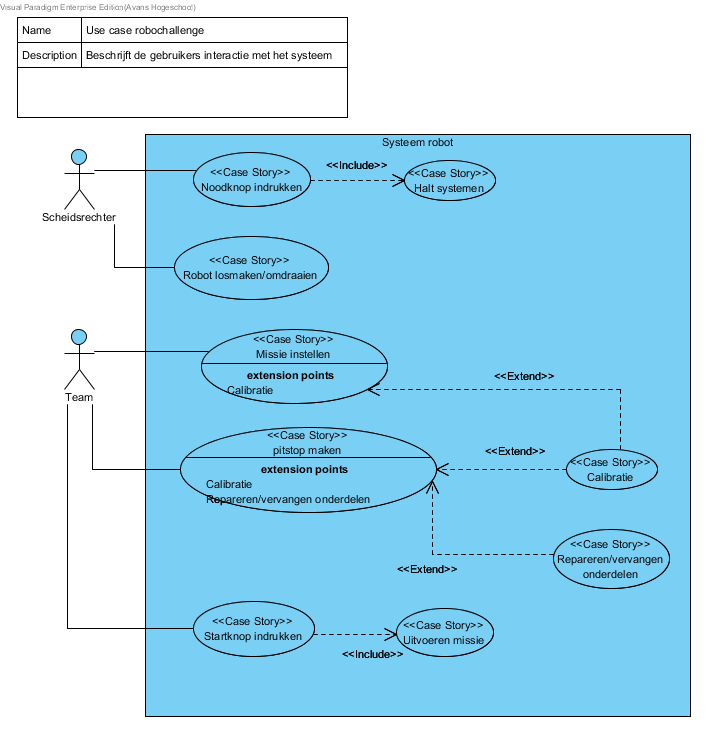
\includegraphics[scale=.9]{usecase.png}
\caption{Use case diagram van het globale systeem}
\label{fig:usecase}
\end{figure}
\end{center}
\clearpage

\subsection{Use case omschrijvingen}

% Table generated by Excel2LaTeX from sheet 'Blad1'
\begin{table}[htbp]
  \centering
  \caption{Use case omschrijving}
    \begin{tabular}{llll}
    \toprule
    Naam Use Case & \multicolumn{3}{l}{\textbf{Robot uitzetten/verwijderen}} \\
    \midrule
    Samenvatting & \multicolumn{3}{l}{In geval dat er iets fout gaat moet de scheidsrechter de robot kunnen deactiveren.} \\
    \multirow{2}[2]{*}{Actoren} & \multicolumn{3}{l}{Scheidsrechter (R)} \\
          & \multicolumn{3}{l}{Systeem (robot (S))} \\
    Preconditie & \multicolumn{3}{l}{De robot maakt een fout, of voert een niet handeling uit die niet is toegestaan.} \\
    \multirow{5}[10]{*}{Acties} & 1     & R:    & Drukt op de noodknop van de robot. \\
          & 2     & S:    & Wordt op halt gezet en zal geen functies meer uitvoeren [1]. \\
          & 3     & R:    & Pakt de robot vast aan de handvaten. \\
          & 4     & S:    & Voert geen acties meer uit [1]. \\
          & 5     & R:    & Wordt van het veld verwijderd. \\
    Uitzonderingen & \multicolumn{2}{l}{[1]} & Nadat de robot op halt is gezet zal hij geen enkele functie meer uitvoeren. \\
    \multirow{2}[2]{*}{Postconditie} & \multicolumn{3}{l}{De robot kan geen functionaliteiten uitvoeren en is door de scheidsrechter van het speelveld verwijdert.} \\
          & \multicolumn{3}{l}{} \\
    Special Requirements  & \multicolumn{3}{l}{Verwijdert uit het veld door omstandigheden die zijn bepaald door de scheidsrechter.} \\
    \bottomrule
    \end{tabular}%
  \label{tab:addlabel}%
\end{table}%
\clearpage

\begin{table}[htbp]
  \centering
  \caption{Use case omschrijving}
    \begin{tabular}{llll}
    \toprule
    Naam Use Case & \multicolumn{3}{l}{\textbf{Missie instellen}} \\
    \midrule
    Samenvatting & \multicolumn{3}{l}{Aan het begin van de missie moet de camera gekalibreerd worden zodat de robot de goede kleur ballen detecteerd.} \\
    \multirow{3}[1]{*}{Actoren} & \multicolumn{3}{l}{Team (T)} \\
          & \multicolumn{3}{l}{Scheidsrechter (R)} \\
          & \multicolumn{3}{l}{Robot (S)} \\
    Preconditie & \multicolumn{3}{l}{De robot staat gedeactiveerd op het speelveld met een willekeurige missie opgesteld.} \\
    \multirow{5}[9]{*}{Acties} & 1     & T:    & Drukt op de aan knop. \\
          & 2     & S:    & Wordt geactiveerd. Wacht op een kleur (papier) voor kalibratie. \\
          & 3     & R:    & Houdt een kleur (papier) voor de camera van de robot. \\
          & 4     & S:    & Herkent de kleur. \\
          & 5     & S:    & Start de missie. [1] \\
    Uitzonderingen & \multicolumn{2}{l}{[1]} & Indien de robot de kleur goed registreert zal hij dit laten weten door middel van een geluid. \\
    \multirow{2}[1]{*}{Postconditie} & \multicolumn{3}{l}{De robot zoekt de gekleurde ballen. Indien de robot gekalibreerd is op deze kleur zal hij de bal grijpen.} \\
          & \multicolumn{3}{l}{} \\
    Special Requirements  & \multicolumn{3}{l}{Heeft een kleur nodig voor kalibratie.} \\
    \bottomrule
    \end{tabular}%
  \label{tab:addlabel}%
\end{table}%
\clearpage

% Table generated by Excel2LaTeX from sheet 'Blad1'
\begin{table}[htbp]
  \centering
  \caption{Use case omschrijving}
    \begin{tabular}{llll}
    \toprule
    Naam Use Case & \multicolumn{3}{l}{\textbf{Pitstop maken voor reparatie}} \\
    \midrule
    Samenvatting & \multicolumn{3}{l}{Dit wordt tussen de missies door gedaan, het team kan op dat moment kalibreren en eventuele reparatie uitvoeren.} \\
    \multirow{2}[1]{*}{Actoren} & \multicolumn{3}{l}{Team (T)} \\
          & \multicolumn{3}{l}{Robot (S)} \\
    \multirow{2}[1]{*}{Preconditie} & \multicolumn{3}{l}{De robot hoeft op het moment geen missie uit te voeren of mee te doen aan een wedstrijd.} \\
          & \multicolumn{3}{l}{De robot heeft een kapotte component.} \\
    \multirow{6}[11]{*}{Acties} & 1     & S:    & Staat in de pitstop voor reparatie. \\
          & 2     & S:    & Is gedeactiveerd. \\
          & 3     & T:    & Zoekt naar het kapotte component. \\
          & 4     & T:    & Vervangt het kapotte component. \\
          & 5     & T:    & Activeert de robot om het component te testen. \\
          & 6     & S:    & Voert een testronde uit. [1] \\
    Uitzonderingen & \multicolumn{2}{l}{[1]} & Indien het kapotte component niet werkt zal het team de stappen 2 tot 5 opnieuw uit moeten proberen. \\
    \multirow{2}[1]{*}{Postconditie} & \multicolumn{3}{l}{De robot werkt weer en kan weer missies gaan rijden.} \\
          & \multicolumn{3}{l}{} \\
    Special Requirements  & \multicolumn{3}{l}{De robot hoeft op dat moment geen missie te rijden.} \\
    \bottomrule
    \end{tabular}%
  \label{tab:addlabel}%
\end{table}%
\clearpage




\newpage

%----------------------------------------------------------------------------------------
% Conclusion?
%----------------------------------------------------------------------------------------
\section{Conclusie}
\label{sec:conclusion}
\lipsum[0-2]
\newpage
%----------------------------------------------------------------------------------------
%	Glossary
%----------------------------------------------------------------------------------------
%\clearpage
%\printglossaries
%----------------------------------------------------------------------------------------
%	Bibliography
%----------------------------------------------------------------------------------------
% \clearpage
% \bibliographystyle{plainurl}
% \nocite{*}
% \bibliography{Bibliography}
%----------------------------------------------------------------------------------------
%	Appendix
%----------------------------------------------------------------------------------------
%\addcontentsline{toc}{section}{Appendix A - Interns' hip assignment}
%\includepdf[pagecommand=\section*{Appendices}\subsection*{Appendix A - Internship assignment} The document including the assignment to the interns from Streamit,pages=-,scale=0.67]{appendices/Internship_assignments.pdf}
%----------------------------------------------------------------------------------------
%	End of document
%----------------------------------------------------------------------------------------
\end{document}

%figure example
%figures~\ref{fig:ganttFig1} and~\ref{fig:ganttFig2}.\\
%\begin{figure}
%\includegraphics{gantt4_2.png}
%\caption{Iterations of the project}
%\label{fig:ganttFig1}
%\end{figure}
%\begin{figure}
%\begin{center}
%%\includegraphics[angle=90,width=\textwidth,height=\textheight,keepaspectratio]{versie4.png}
%\includegraphics[angle=90,width=\textwidth,height=\textheight,keepaspectratio]{gantt4.png}
%\caption{Gantt chart of the planning}
%\label{fig:ganttFig2}
%\end{center}
%\end{figure}